%-------------------------------------------------------------------------------
--------------------------------
%------------------------------------------------- Chapter 1 --------------------------------------------------------
\parskip=0.6cm

\chapter{Introducción}\label{cap:1}
\pagenumbering{arabic}


Esta tesis se inició en el 2005 atendiendo a requerimientos de mayor flexibilidad y dinamismo de los entornos e-learning, planteados por un grupo interdisciplinario de I+D del CONICET-UNR dedicado a problemáticas de integración de las Tecnologías de la Información y Comunicación (TIC) en contextos organizacionales de Educación Superior. 
Dichos requerimientos se enfocaban hacia mejorar la calidad y posibilidades de desarrollo de procesos educativos, de investigación y de producción hipermedial bajo la
modalidad de taller físico-virtual. Esta necesidad permitió la elaboración de las
primeras hipótesis de la presente investigación delimitando los alcances del estudio circunscriptos a la
Ingeniería de Software y Ciencias de la Computación aplicada a la interpretación
de la complejidad de estos requerimientos y su correspondiente
infraestructura de resolución.

El desafío que afrontó este trabajo en todo su trayecto, fue colaborar desde las Ciencias de la Computación al despliegue del diálogo y producción interdisciplinar del grupo de trabajo sobre el campo conceptual referido a la integración de TIC en procesos antes mencionados. 
Así, se fue generando una construcción teórica y metodológica denominada consensuadamente como "Dispositivo Hipermedial Dinámico" -DHD-(P. San Martín, et. al, 2008). Desde la experiencia previa del autor de este trabajo, los requerimientos planteados demandaron realizar un estudio específico de proyectos centrados especialmente en el campo del "e-learning".

De estas indagaciones se adhirió a que los sistemas colaborativos se mostraban como una propuesta racional para sostener modelos
donde se pueden implementar soluciones tecnológicas para requerimientos
funcionales que deriven de un requisito de más alto nivel en los que aumenta
el grado de subjetividad. Esto se presenta  debido a que es necesario tener en cuenta
cuestiones de contexto, tipos de relaciones y vínculos que dan lugar a diferentes
niveles de complejidad y de interpretación. 

Actualmente se evidencia un creciente
interés por metodologías de trabajo más
efectivas, que toman muy en cuenta el potencial de cada uno de los sujetos. Se
busca generar conocimiento útil a partir de
la información disponible y el desarrollo de
competencias que permitan aplicar ese
conocimiento efectivamente. No obstante,
la complejidad de muchos problemas
requiere del trabajo de grupos, constituidos por
personas capaces de interactuar de forma
sinérgica para buscar soluciones adecuadas y con alto grado de creatividad \cite{cap1.1}. La construcción de conocimiento aplicando metodologías de diálogo interdisciplinar ha dejado de ser una
opción para convertirse en una necesidad. Es en este sentido que se sostiene en esta tesis una perspectiva computacional acorde al contexto, totalmente integrada a los postulados del Programa de Investigación, Desarrollo y Transferencia "Dispositivos Hipermediales Dinámicos" radicado en el CIFASIS (CONICET-UNT-UPCAM) bajo la dirección de la Dra. Patricia San Martín. 

Debido al papel protagónico de las TIC en la actual Sociedad de la Información y del Conocimiento y, el vertiginoso desarrollo que
han tenido en los últimos años, se han
planteado paradigmas y esquemas de
trabajo que integran a las ciencias
computacionales con otros campos del
conocimiento tales como las ciencias humanas
y sociales, las ciencias administrativas, el
diseño gráfico y artístico, etc., en un
intento de construcción de un nuevo contexto físico-virtual pero
reconociendo al tiempo, que pese al
potencial de las TIC, gran parte de los problemas
a resolver, no pueden ser
abordados exclusivamente desde una
perspectiva tecnológica \cite{cap1.2,cap1.3}. 

La elección de metodologías y paradigmas en los que se integran tecnologías
y funcionalidades conceptuales, necesitan ser interpretados como posibles
instancias que se pueden configurar. Por lo tanto, se pueden interpretar
propiedades generales de los sistemas a partir de las posibles configuraciones
de un estado determinado, de un caso de uso concreto. Este análisis es tratado en el grupo de I+D "Obra Abierta: DHD para educar e investigar"
a través de la teoría de los sistemas complejos y se tiene en cuenta como
items para la clasificación de aplicaciones ``Groupware''.

Los aspectos que se tendrán en cuenta en esta tesis sobre los sistemas colaborativos son:

Nivel de automatización: Las aplicaciones ``Groupware`` como considera
Patricia Schnaidt, se pueden clasificar de acuerdo al tipo de trabajo en grupo
que apoyan: \cite{{cap1.1.groupware}

\textit{Flujo de documentos, Automatización de procesos, Automatización de
tareas, Herramientas flexibles de trabajo en grupo.}

\begin{itemize}
\item De acuerdo al espacio-tiempo de los miembros del grupo: Se consideran las
aplicaciones “groupware” de acuerdo al tipo de interacción de los miembros del
grupo de trabajo \cite{cap1.4.groupware}.

\begin{itemize}
 \item Interacción Sincrónica:
 \item Interacción Asincrónica:
 \item Distribución Sincrónica:
\end{itemize}

\item De acuerdo al manejo de información. Según el soporte que brindan
\cite{cap1.5.groupware} los sistemas “groupware” pueden clasificarse en:
\begin{itemize}
 \item Sistemas para compartir Información.
 \item Sistemas cooperativos.
 \item Sistemas concurrentes.
\end{itemize}

\item De acuerdo al propósito de la aplicación: es posible encontrar dos tipos de
aplicaciones dependiendo de su propósito.
\begin{itemize}
 \item Aplicaciones de propósito general.
 \item Aplicaciones de propósito específico.
\end{itemize}

\item De acuerdo al tipo de aplicación: Dependiendo del tipo de aplicación
y funcionalidad se pueden clasificar en los siguientes grupos:

\begin{itemize}
 \item Sistemas de mensajes por computador
 \item GDSSs (Group Decision Support Systems).
 \item Sistemas de coordinación: Orientados a la formas, orientados al proceso,
orientados al diálogo, orientados a la estructura de comunicación.	
\end{itemize}

\item De acuerdo al tipo de reconfiguración orientada la Interactividad DHD\cite{libro.unr}. Dependiendo del grado de expresión que se
tiene para reconfigurar el sistema teniendo en cuenta información procesada
para la representación de contexto interno y del entorno.

\begin{itemize}
 \item Reconfiguración dinámica.
 \item Adaptabilidad.
 \item Sensibilidad al contexto.
 \item Sistemas expertos: bases de conocimientos y motores de inferencias.
\end{itemize}

\end{itemize}


Los aportes de originales de la tesis se fundamentan en publicaciones de circulación internacional acreditadas proponiendo una perspectiva innovadora referida a la reconfiguración dinámica de los entornos colaborativos orientada a la Interactividad DHD.


\section{Motivación}\label{sec:motivacion}


A medida que el avance en la investigación y desarrollo de entornos
colaborativos brindan mejoras e innovaciones en herramientas
(videoconferencias, porfolios, wikis, workshops, etc.) y sus respectivos
servicios, crece la cantidad de posibles configuraciones de los espacios
colaborativos.

Estas configuraciones abarcan diferentes tipos de requerimientos pertenecientes
a las  etapas de diseño, desarrollo e incluso exigen que el espacio
colaborativo se ''adapte'' en tiempo de ejecución. A partir de estos
requerimientos iniciales se
definen los procesos e-colaborativos (denominados en esta tesis como
Pe-colaborativos) \cite{cacic2007.7} de manera semejante a procesos de negocio
en otros dominios de
aplicación. Esta denominación parte de la evolución del recorrido
teórico inciado a partir de las transacciones Web, que dieron lugar a
teorizar el concepto de transacciones e-learning \cite{cacic2007} y que en el trayecto de desarrollo de esta investigación evolucionaron finalmente hacia el concepto de
procesos e-colaborativos. 

Al igual que los procesos de negocios en una Aplicación Web
convencional, los Pe-colaborativos están compuestos por transacciones Web
\cite{cacic2007.7}. En este contexto, una transacción (o transacción
e-colaborativa) es definida como una secuencia de actividades que un usuario
ejecuta a través de una Aplicación colaborativa con el propósito de efectuar una
tarea o concretar un objetivo, donde el conjunto de actividades, sus propiedades
y las reglas que controlan sus ejecuciones dependen del Pe-colaborativos que la
Aplicación debe brindar. Un ejemplo de esto es la posibilidad de implementar una estrategia didáctica que le brinde a un alumno que participa en un entorno virtual colaborativo la posibilidad de acceder a un tipo de Objeto Digital Educativo, dependiendo de sus intervenciones en los Foros. 
Estos requerimientos resultan difíciles de implementar en las actuales aplicaciones e-learning de
extendido uso a nivel global.

Las características funcionales de aplicaciones Web
colaborativas (AW-Colaborativas), como
Sakai \footnote{\url{http://sakaiproject.org/}}, se basan en brindar
navegación entre páginas a través de links y ejecución de transacciones
colaborativas  desde las herramientas (ej., Foros, Anuncios, Exámenes, Blogs,
etc.) que utilizan los servicios de la plataforma (ej., edición, manejo de audio
y vídeo, consultas, navegación, etc.).

En el marco de los análisis efectuados se observó que el proyecto Sakai
brinda una de las propuestas más consolidadas de diseño y desarrollo de
entornos colaborativos, teniendo en cuenta los anteriores items
\ref{sec:motivacion} analizados.

Sakai está orientado a herramientas que se implementan a través de servicios
comunes (servicios bases). Por ejemplo, el servicio de edición de mensajes es
utilizado en las herramientas Foro, Anuncio,Blog, PorFolio, etc. Más aun, otras
de las características salientes de Sakai es la versatilidad para su extensión
y/o configuración que permite alterar ciertas configuraciones  en
tiempo de ejecución, por ejemplo, instrumentar una nueva funcionalidad en un
servicio base de Sakai.

Sin embargo, estas soluciones no pueden resolver aquellos Pe-Colaborativos que
involucren cambios en el comportamiento de la relaciones entre un componente
(cliente) que ocasiona, a través de un pedido, la ejecución de un componente
servidor (proveedor). Estos cambios refieren a la capacidad de
adaptación dinámica del sistema \cite{cacic2007.14} extendiendo, personalizando
y mejorando los servicios sin la necesidad de recompilar y/o reiniciar el
sistema. 

Esta tesis doctoral presenta una propuesta para la incorporación (agregado) de
propiedades  de adaptación dinámicas, reconfiguración e inteligencia
(AdRI) \label{AdRI} a los servicios bases del framework Sakai,
especialmente diseñadas para implementar Pe-Colaborativos definidos en el marco
de \cite{cacic2007.9} donde se requieren nuevos aspectos de adaptación
\cite{librounq} implementados a partir del framework Sakai. Dicha
implementación se ajusta a los requisitos y requerimientos
(capítulo \ref{cap:1}) del Dispositivo
Hipermedial Dinámico, que como red sociotécnica responsable posibilita a los sujetos desarrollar actividades académicas y profesionales bajo la modalidad de taller físico-virtual.  

Cuando se refiere a las propiedades de inteligencia de un framework, se atribuye a un entorno con características  heterogéneas con numerosos
componentes de software y hardware \cite{cap1.133}. Esta diversidad implica ciertos
desafíos problemáticos que demandan una atención especial en los diseños solicitando una preparación para usos compejos multisensoriales:

\begin{itemize} 
 
\item
Se han de integrar y gestionar distintos tipos de tecnología, con
el consecuente aumento de complejidad en el desarrollo. El usuario puede
utilizar múltiples modos (habla, gestos, tacto, etc.) para interaccionar con
el entorno, con lo que se requieren interfaces de usuario muy variadas. Por
otro lado la distribución de la información requiere distintos tipos de redes,
según la naturaleza de ésta.

\item
Los componentes pueden estar altamente distribuidos. Tanto los
sensores, que se encargan de recoger la información del entorno, como los
actuadores, que transmiten la respuesta del entorno al usuario, pueden
tener localizaciones distribuidas. Nuevamente se añade una dificultad extra a la
hora de desarrollar aplicaciones.

\item
La configuración del entorno es dinámica. No se puede prever siempre
el momento en que se conectan y desconectan nuevos dispositivos o entran
y salen nuevos usuarios.

\item
El sistema tiene que estar funcionando siempre. Esto quiere decir que se
deben evitar la mayor cantidad posibles de tareas en tiempo de compilación. En
este sentido se ven afectados cuestiones de diseño, arquitectura e
implementación que permitan la mayor versatilidad para la ejecución de
cambios en tiempo de ejecución. Además, es importante tener en cuenta
previamente, cuáles van a ser las componentes de los sistemas y qué lugares
ocupan para prepararlas para el cambio o reconfiguración dinámicas. 

\end{itemize}

La combinación de las aplicaciones sensibles al contexto y los entornos activos
conlleva una serie de dificultades adicionales. A la información contextual
generada por usuarios, dispositivos y aplicaciones hay que añadir el contexto
del entorno.

Dentro de un entorno activo se pueden encontrar fuentes de información
contextual de diversa naturaleza. Las fuentes pueden ser muy cercanas al mundo
físico, o por el contrario pueden estar relacionadas con el mundo virtual. El
primer conjunto se compone de toda clase de dispositivos ligados al entorno que
interaccionan con el mundo físico tales como sensores, conmutadores,
electrodomésticos, pantallas, micrófonos, altavoces, etc. El segundo conjunto
incluye aquellos componentes puramente computacionales, tales como gestores de
diálogos, agentes inteligentes, clientes de correo, etc. Ya se ha mencionado la
naturaleza distribuida de estos componentes, lo cual implica mayor complejidad
en el desarrollo de aplicaciones.

Un problema importante surge por la diferencia en cuanto al nivel de abstracción
en la información contextual aportada por los distintos componentes. Los
sensores manejan información de alta resolución que es rica en detalles pero
pobre en cuanto a abstracción. En cambio las aplicaciones pueden requerir
información contextual más elaborada que la que aportan los sensores. Los
desarrolladores tienen que convivir con información que tiene distinta
resolución, lo que implica distintos formatos y distintas redes de
distribución.

Finalmente, la interfaz de comunicación con el usuario debe ser lo más flexible posible, para
promover la interactividad tanto en los aspectos comunicacionales como de acceso y edición de información que permiten actualmente las TIC. El logro de una integración natural de estas tecnologías a las actividades cotidianas de los usuarios es un fin representativo de la posibilidad de construcción de un nuevo contexto físico-virtual (capítulo \ref{cap:2}).

Retomando aspectos de I+D, es fundamental que la interfaz tenga el suficiente nivel
de expresión para que se puedan instrumentar adecuadamente las reconfiguraciones
dinámicas, ya que en ellas se encuentra la máxima complejidad
funcional. En este punto el contexto también juega un papel importante, ya que es claro que la
interacción sujeto-ordenador no es tan efectiva como la comunicación intersubjetiva donde se ponen en juego un sinnúmero de posibilidades de interacción entre los sujetos y en relación al contexto. 
En la mayoría de los casos resulta una adecuación forzada del sujeto a la máquina, solución contrapuesta a lo que se espera de una tecnología interactiva.

Para subsanar esta contradicción, se ha señalado que un punto importante es determinar cuál es la
información contextual que el usuario debe suministrar al sistema para
conseguir una mejor interacción. Entonces, una vez determinado el contexto, es
preciso capturarlo. Esto requiere de múltiples sensores e interfaces de
tal forma que se pueda captar tanto la interacción explícita como la implícita
del usuario, teniendo en cuenta que este proceso se realice de
forma no intrusiva.  

Tal como se deduce del título \footnote{Contratos Sensibles al Contexto
para el Dispositivo Hipermedial Dinámico} el planteamiento de esta tesis
tiene en cuenta el contexto como una componente de primera clase.

Ahora bien, el término información contextual tiene múltiples acepciones
que dependen del dominio de aplicación. Incluso si se restringe éste al campo de
las Ciencias de la Computación, se registra aún un amlio espectro de posibles definiciones. En la presente tesis se considera el contexto en el mismo sentido
que le dan los trabajos realizados en aplicaciones sensibles al contexto. Esta
área engloba aplicaciones y dispositivos que consideran como una entrada más del
sistema la información sobre las circunstancias bajo las cuales operan. Estas
circunstancias pueden ser la localización, la tarea que está realizando el
usuario, otros recursos que se encuentren cercanamente, las condiciones ambientales del
entorno, etc. La definición y representación del contexto es un punto central de
este trabajo que se tratará en profundidad en el capítulo \ref{cap:3} teniendo en
cuenta que el contexto para el DHD necesita un tratamiento específico. 

El alcance del estudio queda acotado a las aplicaciones sensibles al contexto
que operan dentro de un entorno inteligente. Este consiste en una
infraestructura restringida por unas barreras físicas y compartida por un
conjunto de aplicaciones, dispositivos y sujetos. El adjetivo inteligente se
emplea para indicar la habilidad de adquirir información de forma autónoma y de
emplearla para adaptarse a las necesidades de los sujetos intervinientes. El
entorno se convierte en una aplicación sensible al contexto más, contribuyendo
activamente en la interacción con el usuario. Así, en la literatura también se
pueden encontrar referencias a los entornos inteligentes como entornos activos
(``Active Environment``) o espacios activos (''Active Spaces''). Un
hogar, una oficina, una clase, un vehículo o un restaurante son ejemplos
posibles de entornos activos. 

Para situar la importancia del contexto y su relación con los entornos
inteligentes es necesario referirse a la Computación Ubicua, una tercer área de
investigación que engloba a los dos temas centrales de la tesis. La Computación
Ubicua \ref{cap1.6}, también es conocida como Computación Pervasiva (``Pervasive
Computing``) Ya Mark Weiser (1993), propone trasladar la capacidad de computación de
los rígidos y voluminosos ordenadores personale de la época a miles de dispositivos
diseminados por el entorno, de forma que las computadoras puedan fundirse con el
entorno hasta volverse invisibles al usuario.

Esta perspectiva dan lugar a requerimientos centrados en el logro del máximo
posible nivel de encapsulamiento para los procesos de reconfiguración
dinámica y usos de servicios reconfigurados. O sea que los usuarios no deberían acceder a cómo están
implementadas las reconfiguraciones y su habilitación para el uso. De alguna
manera esto determina alcanzar un nivel de transparencia hacia el usuario que
está mediado por el tipo de tecnología. En este sentido para alcanzar
niveles óptimos de transparencia será necesario aún un salto tecnológico
importante. Dicho según las palabras de Donald Norman \cite{cap1.196}:

\begin{quote}
Necesitamos movernos hacia la tercera generación de ordenadores
personales, la generación donde la máquina desaparece de la vista,
donde podemos volver a concentrarnos en las actividades y objetivos
de nuestra vida.
\begin{flushright} Donald Norman \end{flushright}
\end{quote} 

Hay tres transformaciones que devienen de la Computación Ubicua en las
aplicaciones informáticas que también se deben tener en cuenta cómo
condiciones a respetar. Estas transformaciones fundamentan las decisiones del uso de
aplicaciones Web sobre las de escritorio.

\begin{itemize}
 
\item Reconocer el contexto. 

Uno de los puntos débiles de las aplicaciones de escritorio es la insensibilidad
ante los cambios de contexto del usuario.
Mientras que se registra un considerable avance en la modelización del usuario
y la adaptación según diferentes perfiles y preferencias, las aplicaciones
tradicionales muestran el mismo comportamiento independientemente de la
situación en que se encuentre el usuario. El contexto se ha reconocido como
una parte fundamental de la comunicación humana \cite{cap1.69}, por lo que
debe ser incorporado también en el diseño de los sistemas informáticos para
acercarlos a los códigos humanos de comunicación. La localización, la actividad o
el foco de atención del usuario, entre otras variables contextuales tienen que
formar parte de las nuevas aplicaciones ubicuas.

\item Actuar proactivamente. 

El diálogo entre la aplicación y el usuario puede
ser iniciado o bien por el usuario, o bien por la aplicación, o bien una
mezcla de ambos. En general, la mayor parte de las aplicaciones de escritorio
son pasivas, ya que es el usuario el que debe tomar la iniciativa. Un
campo que ha prestado especial interés por la proactividad son los agentes
personales. Éstos se encargan de buscar y mostrar información según la
preferencias del usuario pero sin necesitar supervisión explícita. En el marco
de la Computación Ubicua es preciso introducir en el diseño de las aplicaciones
cierto grado de proactividad que permita liberar la atención del usuario
cuando no sea imprescindible. Para ello se hace necesario realizar modelos
del comportamiento humano \cite{cap1.198} que permitan inferir las
necesidades del usuario.

\item Funcionalidades ubicuas. 

Actualmente para que una aplicación sea ubicua
es necesario instalarla en cada uno de los dispositivos donde se quiere emplear,
teniendo en cuenta que para cada dispositivo se cargará una versión distinta que
se ajuste a las restricciones que éste imponga. Esto incrementa la complejidad
en el desarrollo, mantenimiento e interoperatibilidad de las diferentes
versiones de la aplicación. Una aproximación para solucionar este problema es
mantener una funcionalidad única y generar la interfaz dinámicamente adaptándose
a lo que requiera el usuario en cada momento \cite{cap1.205}. En este
sentido se están realizando importantes esfuerzos por estandarizar lenguajes de
representación de interfaces de usuario abstractas como UIML \cite{cap1.16} o
XIML \cite{cap1.214}, de modo que se pueda definir una interacción genérica
independiente del modo a emplear y ligarla dinámicamente con la funcionalidad.
\end{itemize}

La consecución de estos objetivos recae sobre tres tecnologías: la computación
ubicua, las aplicaciones sensibles al contexto y los entornos inteligentes.
Recientemente, a la combinación de estas tres áreas se le ha denominado
Inteligencia 
Ambientad\footnote{
Documento donde por primera vez se introduce el concepto y definición de
"Inteligencia
Ambiental"  \url{http://www.epstein.org/brian/ambient_intelligence.htm}}. Esta
se refiere a la presencia de un entorno digital
que es interactivo, sensible, y adaptativo a la presencia de sus ocupantes
\cite{cap1.16}.

La Inteligencia Ambiental pretende fundir los conceptos de ubicuidad y
transparencia en un diseño centrado en el usuario que dé como resultado un
verdadero ordenador invisible. Para esta tesis, esta premisa es tenida en
cuenta para la elección de propuestas tecnológicas externas utilizadas en las
implementaciones. Esto quiere decir, que no se abordará la problemática de
formar Ambientes Inteligentes a partir de dispositivos físicos. La intención se centra en tomar alguno de los fundamentos para aplicarlos en el tipo de
propuesta de solución que se persigue. Se promueve el diseño centrado en el usuario y el uso de sistemas altamente interactivos. El objetivo
final es conseguir que las tecnologías previamente mencionadas ayuden de manera
no invasiva al desarrollo de procesos para educar, investigar y producir mediatizados por el DHD.

\section{Solución propuesta y contribución} \label{solución}

La propuesta de solución a los requerimientos mencionados sobre
Adaptación dinámica, Reconfiguración e Inteligencia (AdRI) está enfocada a la
inyección de una nueva componente dentro de un sistema tecnológico origen. Esta
componente a su vez está conectada con nuevos subsistemas que de forma
estratificada se incorporan al original. Una posible representación de esta
interpretación se describe en la figura \ref{fig:solucion} para colaborar en la comprensión sobre cuál es la estructura en la que se basa la propuesta de
solución.


\begin{figure}[h]
\begin{center}
 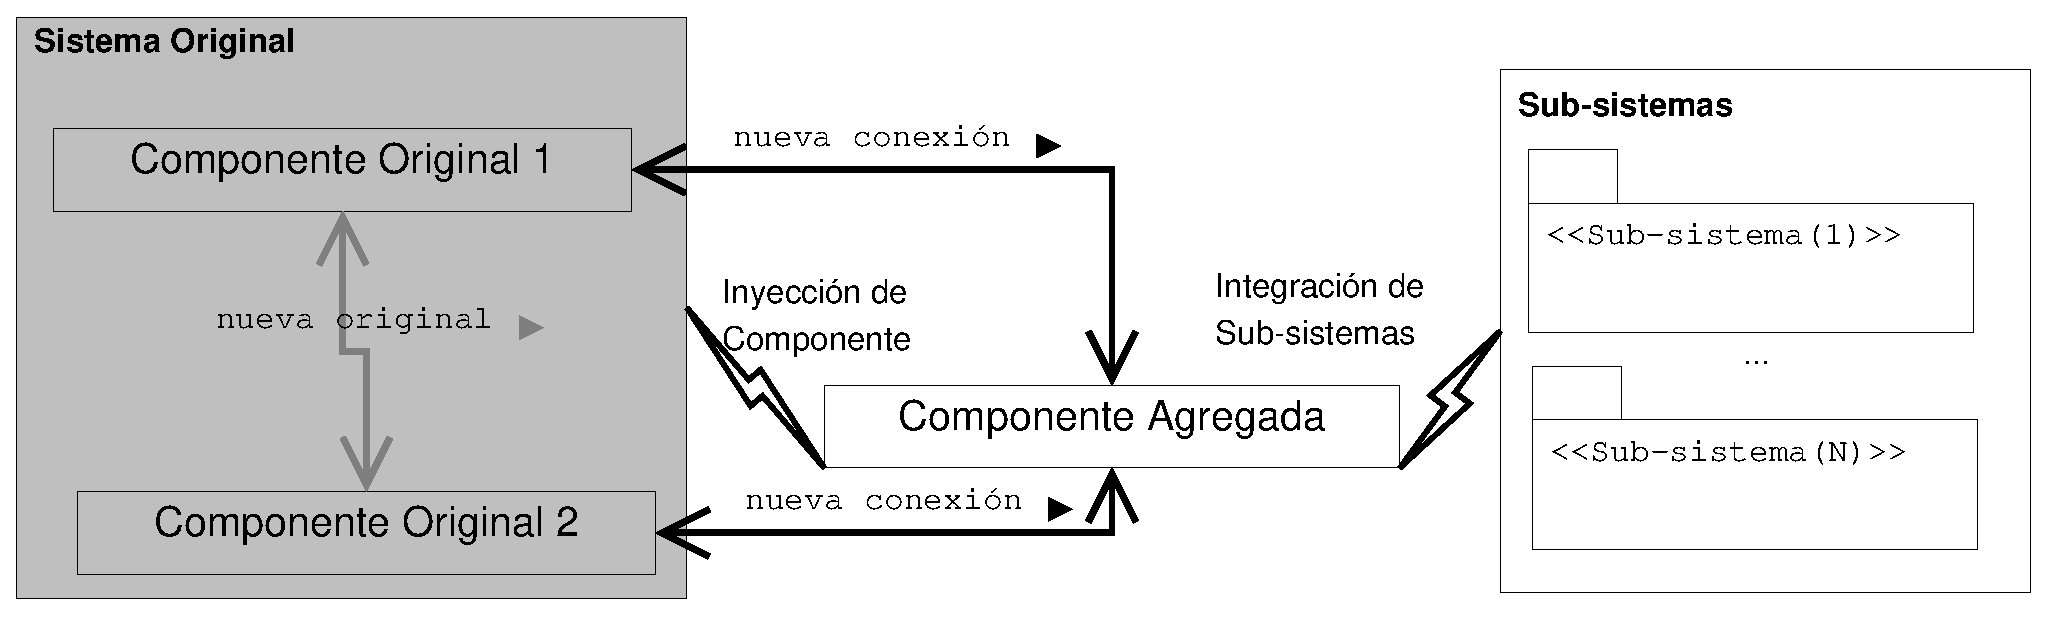
\includegraphics[width=4 in,totalheight=3 in] {Ch0/solucion}
 % .: 0x0 pixel, 0dpi, 0.00x0.00 cm, bb=
\caption{Estructura de la solución} \label{fig:solucion}
\end{center}
\end{figure}

La parte gris de la figura representa las componentes de un sistema original
con sus componentes y relaciones. Luego se representa el agregado de una nueva
componente (\textit{componente agregada}) que se relaciona con las
\textit{componentes originales} del sistema por medio de \textit{nuevas
conexiones}. Esta nueva relación se denomina \textit{inyección de componentes}.
Luego la \textit{componente agregada} se conecta con diferentes subsistemas. De
esta manera queda conformado un nuevo sistema a partir del
original, proponiéndose una "estructura de la solución para
el DHD" (EstDHD).

En este caso, la componente agregada es el comienzo de la
construcción de un modelo de contrato orientado a la implementación de servicios
sensibles al contexto. El uso de contratos parte de la noción de Programación
por Contrato (”Programing by Contract”) de Meyer \cite{cap1.11} basada en la
metáfora de que un elemento de un sistema de software colabora con otro,
manteniendo obligaciones y beneficios mutuos. En el dominio de aplicación cabe
considerar que un objeto cliente y un objeto servidor “acuerdan“ a través de
un contrato (representado con un nuevo objeto) que el objeto servidor satisfaga
el pedido del cliente, y al mismo tiempo el cliente cumpla con las condiciones
impuestas por el proveedor.

Como ejemplo de la aplicación de la idea de Meyer en un dominio de
sistema colaborativo e-learning se expone la situación en que un
usuario (cliente) utiliza un servicio de edición de mensajes (servidor) a través
de un contrato que garantizará las siguiente condiciones: el usuario debe poder
editar aquellos mensajes que tiene autorización según su perfil (obligación del
proveedor y beneficio del cliente); el proveedor debe tener acceso a la
información del perfil del usuario (obligación del cliente y beneficio del
proveedor).

A partir de la conceptualización de contratos según Meyer se propone una
extensión por medio del agregado de nuevas componentes para instrumentar
mecanismos que permitan ejecutar acciones dependiendo del contexto (figura
\ref{fig:solucion}).

En aplicaciones sensibles al contexto \cite{cap1.6}, el contexto (o información
de contexto) es definido como la información que puede ser usada
para caracterizar la situación de una entidad más allá de los atributos que la
definen. En un caso del campo educativo, una entidad es un usuario (alumno, docente, etc.),
lugar (aula, biblioteca, sala de consulta, etc.), recurso (impresora, fax, etc),
u objeto (examen, trabajo práctico, etc.) que se comunica con otra entidad a
través del contrato. En \cite{cap1.2} se propone una especificación del concepto
de contexto partiendo de las consideraciones de Dourish \cite{cap1.20} y
adaptadas al dominio de sistemas colaborativos con funcionalidades e-learning,
que se consideran en este trabajo.

Contexto es todo tipo de información que pueda ser censada y procesada, a través
de la aplicación (por ejemplo, una aplicaión colaborativa e-learning), que
caracterizan a un usuario o entorno, por
ejemplo: intervenciones en los foros, promedios de notas, habilidades, niveles
de conocimientos, máquinas (direcciones ip) conectadas, nivel de intervención en
los foros, cantidad de usuarios conectados, fechas y horarios, estadísticas
sobre cursos, etc.

En términos generales, la coordinación de contratos es una conexión
establecida entre un grupo de objetos aunque en los límites de este trabajo sólo se consideran
dos objetos: un cliente y un servidor.

Cuando un objeto, cliente efectúa una llamada a un objeto servidor (ej., el
servicio de edición de la herramienta Foro), el contrato ”intercepta” la
llamada y establece una nueva relación teniendo en cuenta el contexto del
objeto cliente, el del objeto servidor, e información relevante adquirida
y representada como contexto del entorno [20]. Como condición necesaria, el uso
de contratos no debe alterar la funcionalidad de la implementación de los
objetos participantes, aunque sí se espera que altere la funcionalidad del
sistema.

A continuación se presenta sintéticamente un modelo conceptual de contratos sensibles
al contexto de donde se infieren las distintas soluciones propuestas en esta
tesis. Se brindarán detalles sobre algunos de los componentes y relaciones
esenciales para la integración de este modelo con el framework colaborativo que
se identifica con la parte gris de la figura \ref{fig:solucion} y algunos de
sus sub-sistemas representados.


\subsection{Primera noción de los elementos intervinientes en la solución}

Un contrato que siga las ideas de Meyer contiene toda la información
sobre los servicios que utilizarán los clientes. Para incorporar sensibilidad
al contexto los contratos deberán tener referencias sobre algún tipo de
información de contexto que posibilite su utilización.

En el diagrama de relaciones entre entidades analizado en la Figura
\ref{fig:contratosv1} se presenta una primera descripción de los elementos
que componen el concepto de contrato sensible al contexto. A lo largo de la
tesis este mismo diagrama será utilizado para describir diferentes aspectos de
una misma solución. 


\begin{figure}[h]
\begin{center}
 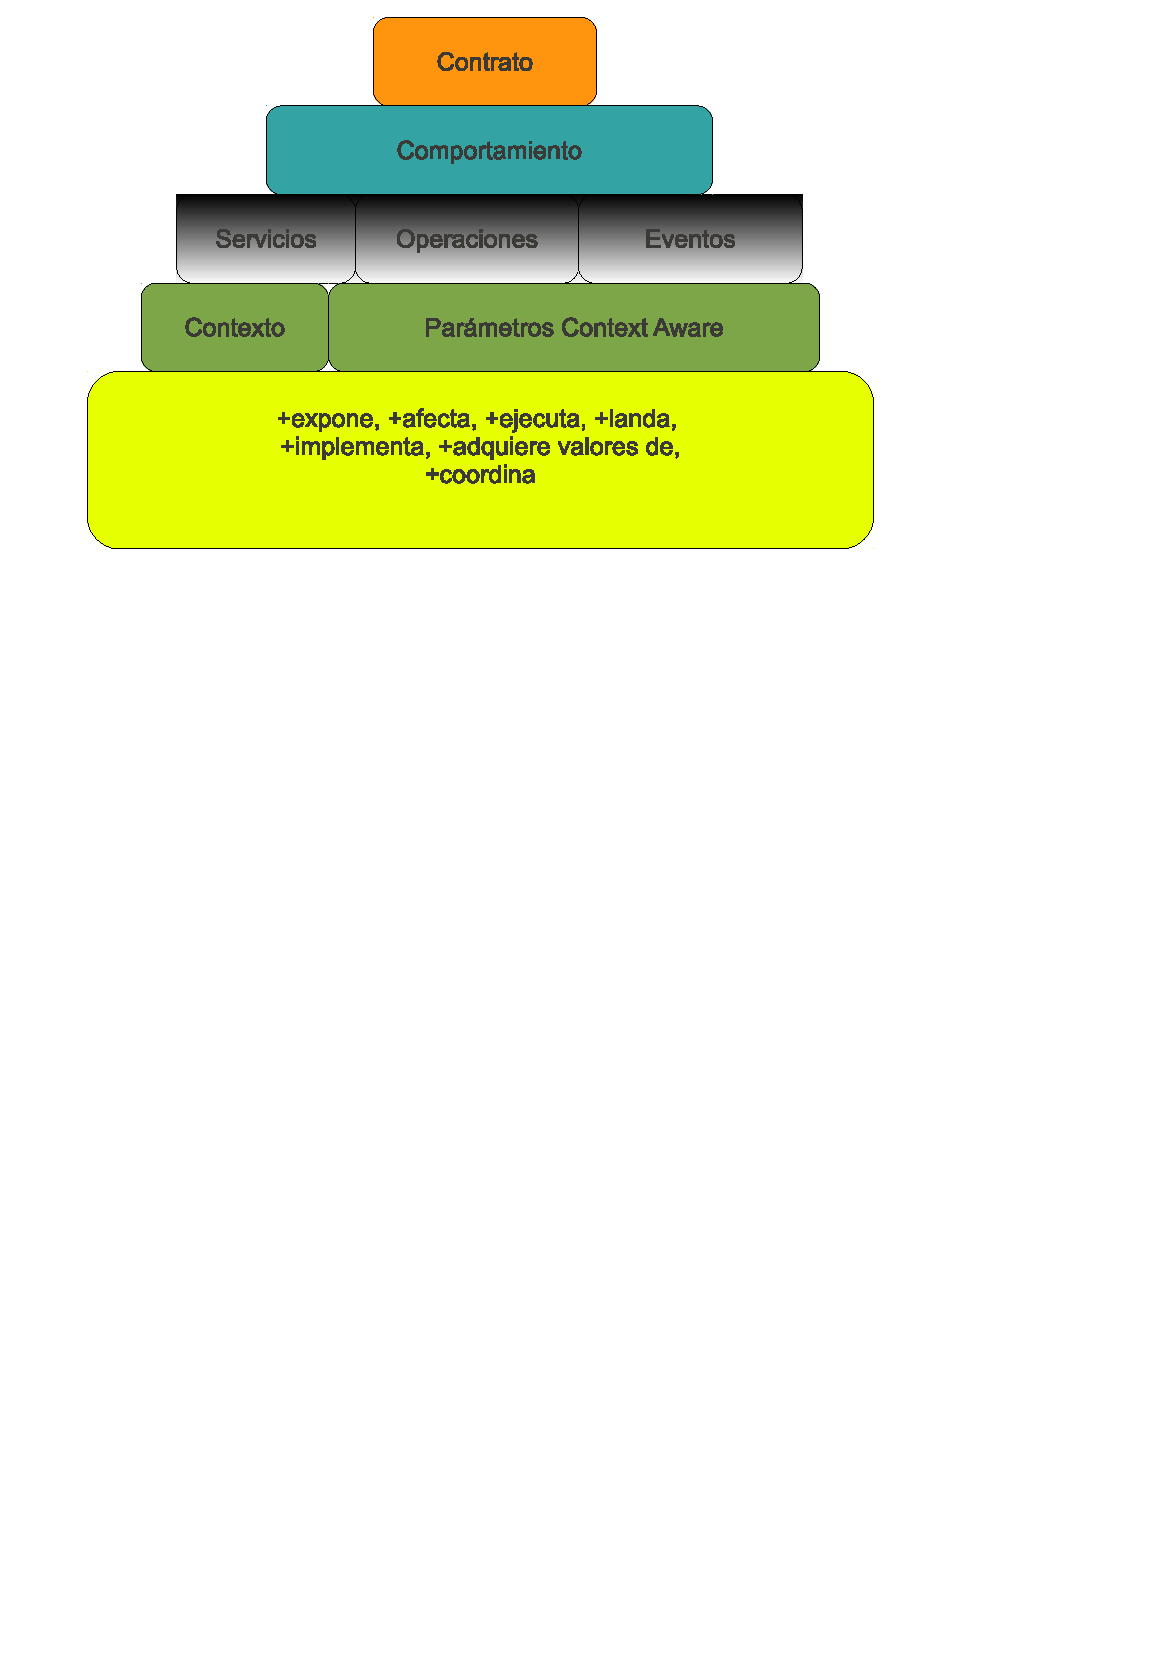
\includegraphics[width=4 in,totalheight=3 in] {Ch0/contratosv1}
 % .: 0x0 pixel, 0dpi, 0.00x0.00 cm, bb=
\caption{Primera interpretación de contratos} \label{fig:contratosv1}
\end{center}
\end{figure}


La configuración de este diagrama se centra en las etapas de diseño e
implementación de diferentes modelos de integración con sub-sistemas
(capítulos \ref{cap:5, cap:6, cap:7}). 


En la figura se muestran los elementos tenidos en cuenta
para la instrumentación de la noción de contrato. Cada uno de los bloques
apilados (desde el pilar 1 al pilar 5) en forma de piramidal pueden representar
componentes abstractas o concretas. En el bloque base se encuentran las
relaciones que  intervienen entre las componentes superiores (pilar 1). Luego
aparecen los bloques de contexto y parámetros context-aware (pilar 2), que
permitirán configurar relaciones que posibilitan resolver requerimientos de
adaptación. Seguidamente se encuentran los bloques que identifican componentes concretas que
integran las herramientas colaborativas (pilar 3) que están sujetas a
modificaciones para establecer las relaciones del bloque base para que se incorporen los
elementos intermedios (pilar 2). Los últimos dos pilares tienen que ver con el
comportamiento (pilar 4) que implementan los pilares inferiores, el contrato
(pilar 5) representa la pieza de software que permitirá el control externo. 

A continuación se presenta la descripción individual de las componentes más importantes:

\textbf{Servicios}: En esta componente se representan los elementos necesarios
para la identificación de un servicio y clasificación de los servicios que
pueden formar parte de las acciones de los contratos. Por ejemplo, nombre del
servicio, identificadores, alcance, propósito, etc. Para más detalles
consultar \cite{cap1.5}. El comportamiento funcional de cada servicio se
expone a través de la componente Comportamiento.

\textbf{Comportamiento}: El comportamiento de un servicio se logra a partir de
combinar operaciones y eventos que son representados por las componentes
Operaciones y Eventos. 

\textbf{Parámetros Context-Aware}: Se denomina parámetros context-aware a la
representación de la información de contexto que forma parte de los
parámetros de entrada de las funciones y métodos exportados por los servicios,
estableciendo de esta manera una relación entre el componente Servicios y el
componente Parámetros contex-aware. La influencia de estos parámetros en el
comportamiento funcional de los servicios es representada a través de
la relación entre los componentes Parámetros context-aware y Comportamiento.

\textbf{Contexto}: Este componente representa el contexto o información de
contexto definida anteriormente en esta sección. Para el modelo planteado en esta tesis, este tipo
de información es utilizada de dos maneras diferentes: 1. para la
asignación de los valores que toman los Parámetros context-aware; 2. esta información puede ser utilizada para definir los invariantes que se
representan en los contratos.

Otro de los elementos importantes que se tendrán en cuenta para la
propuesta de solución es el tipo de representación que se
determina para el entorno. Para este propósito se observará que ligado al
entorno se provea una infraestructura que permita distribuir el contexto
producido por las fuentes. Esta infraestructura fue denominada capa de contexto,
y sirve de intermediaria entre las fuentes contextuales y los elementos que
permitirán  inyectar las propiedades de sensibilidad al contexto del DHD.


\section{Limitaciones}	

Las principales limitaciones que se evidencian en el aporte de esta tesis se relacionan con la formalización de varias de las especificaciones que aquí se
proponen. En este sentido, es necesario iniciar la formalización de los
requerimientos de manera efectiva para captar aquellos aspectos conceptuales
que determinan configuraciones particulares del DHD. Actualmente se cuenta con
un recorrido en la investigación significativo en la construcción de las
especificaciones del DHD, esto se desarrolla en el capítulo
\ref{cap:2} donde se citan modelos canónicos que interpretan propiedades
bien definidas para su descripción formal. 

En el trayecto del textual de la tesis se hace más presente que las problemáticas sobre adaptabilidad dinámica, reconfiguración e inteligencia
(AdRI) están fuertemente orientadas a la construcción de reglas, lo cual
implica que eventualmente pueden existir limitaciones importantes para su
manipulación. En este sentido, el estudio está enfocado en cuestiones de
diseño e implementación en las que se puedan lograr instancias del sistema
cuya configuración resuelva cuestiones funcionales manteniendo las
características de AdRI descriptas en las secciones \ref{motivacion}
y \ref{solucion}.


\section{Organización del documento}

\begin{description}
 \item[Capítulo 1:]
 \item[Capítulo 2:]
 \item[Capítulo 3:]
 \item[Capítulo 4:]
 \item[Capítulo 5:]
 \item[Capítulo 6:]
 \item[Capítulo 7:]
 \item[Capítulo 8:]
 \item[Apéndice:]
 \item[Bibliografía:]
\end{description}


\section{Publicaciones de Apoyo}

La mayor parte de los avances de esta tesis ya fueron publicados en
libros prologados, revistas con referato y memorias de conferencias y
congresos, registrándose a la fecha algunas publicaciones en prensa o revisión.

Los primeros aportes, donde se comienza a desarrollar una noción
sobre la inyección de contratos en una plataforma e-learning, se describe en
el capítulo "Implementaciones de entornos e-learning en la formación de
arquitectos. Hacia una aplicación contex-aware dinámica físico-virtual" Capítulo
XIII en Rodríguez Barros, Diana. (Comp.) Experiencia Digital. Usos, prácticas y
estrategias en talleres de arquitectura y diseño en entornos virtuales. Mar del
Plata, Universidad de Mar del Plata, 2006, pp. 195-204.

El marco teórico y metodológico interdisciplinar que fundamenta la construcción del concepto DHD fue publicado en el
libro: Hacia un Dispositivo Hipermedial Dinámico:
Educación e investigación para el campo audiovisual interactivo \cite{librounq},
cuya autora es la Dra. Patricia San Martín con la colaboración del autor de esta tesis conjuntamente con Griselda Guarnieri y Guillermo Rodriguez. En el capítulo 5 titulado "Sistemas
Context-Aware en dispositivos hipermediales dinámicos para educación e
investigación" se describe una primera aproximación de la arquitectura
conceptual de un DHD con propiedades de sensibilidad del contexto. En el
capítulo 6 titulado "Los contratos context-aware en aplicaciones para educación
e investigación" se introduce la primera noción de los contratos sensibles al
contexto y se propone un mecanismo de implementación. 

Las siguientes dos publicaciones completan el recorrido sobre al
conceptualización del DHD. Fueron tomadas como punto de partida
para la definición de los requerimientos del DHD, propuesto en el capítulo
\ref{cap:2} 

San Martín, P.; Guarnieri, G; Rodirguez, G; Bongiovani, P.; Sartorio, A. ―El
Dispositivo Hipermedial Dinámico: Campus Virtual UNR, publicado en el 2010 por
la Universidad Nacional de Rosario. Este libro, prologado por la Dra.
Graciela Carbone, plantea un proceso de reconceptualización del Campus Virtual
de la Universidad Nacional de Rosario (UNR), Argentina realizado en el marco del
Programa de Investigación, Desarrollo y Transferencia "Dispositivos
Hipermediales Dinámicos" (CIFASIS: CONICET, UNR, UPCAM) a solicitud de la
Secretaría de Tecnologías Educativas y de Gestión (UNR). El objetivo se centró
en promover y fortalecer estratégicamente la integración de las TIC
en actividades educativas, de investigación y vinculación tecnológica en el
actual contexto físico-virtual. La metodología implementada estudió el caso
conjuntamente con los propios actores de la UNR, fundamentándose en conceptos,
método y bases epistemológicas de la investigación interdisciplinaria en el
marco de los sistemas complejos.

San Martín, P.; Guarnieri, G.; Sartorio, A.; Rodríguez, G. ―Construir un campus
virtual: reflexiones sobre un caso de vinculación tecnológica. Publicado en el
2008 por la Revista de la Escuela de Ciencias de la Educación. Este artículo con referato
presenta una de las primeras experiencias de implementación de la modalidad de
becario e investigador en empresa ofrecida por el Consejo Nacional de
Investigaciones Científicas y Técnicas -CONICET-, llevada a cabo durante los
años 2006 y 2007 en una organización que si bien era de base tecnológica,
deseaba consolidar su perfil como institución educativa, ya que sus servicios
principales se centraban desde el año 2000, en la capacitación profesional para
la operatoria de softwares multimediales, desarrollo aplicaciones hipermediales
y composición hipermedial.


Otras publicaciones que colaboraron el conceptual del DHD fueron:

Guarnieri G., Rodríguez G., Sartorio A. (2007). De la máquina de Enseñar
a las Interacciones Múltiples. Congreso sobre nuevas tecnologías y educación
(Edutec 2007), Buenos Aires, Argentina.

Rodríguez G., Sartorio A., Guarnieri G. (2007). El software libre en el
campo del e-learning. Congreso sobre nuevas tecnologías y educación (Edutec
2007). Buenos Aires. Argentina.

San Martín P., Sartorio A., Rodríguez G. (2006) Una mesa de arena para
Investigar y Aprender en Contextos físicos-virtuales-interactivos-comunicacionales de Educación Superior. Actas del
XV Encuentro Internacional de Educación a distancia. UDGV. Guadalajara, México.

Sartorio A., Guarnieri G. (2006), Diseño de herramientas de Context
Aware Dinámico aplicadas a una experiencia de taller físico-virtual-interactivo-comunicacional. Segunda edición de las
Jornadas Abiertas de Informática SADIO Rosario.

En cuanto al recorrido sobre la teoría de los contratos sensibles al contexto,
su implementación y metodología de aplicación, las siguientes
publicaciones (en órden de importancia) sostienen lo expuesto a
partir del capítulo \ref{cap:arqdhd}.

Sartorio, A., Cristiá, M. (2009). First Approximation to
DHD Design and Implementation. CLEI ELECTRONIC JOURNAL.

Rodriguez G., San Martín,P., Sartorio A. (2009),
Aproximación al modelado del componente conceptual básico del Dispositivo
Hipermedial Dinámico. XV Congreso Argentino de Ciencias de la Computación.  

Sartorio A., San Martín P.,  Rodriguez G., Guarnieri
G. (2009),  Los contratos sensibles al contexto para los Dispositivos
Hipermediales Dinámicos. Jornadas de Ciencias de la Computación - FCEIA - UNR.

Rodriguez G., Sartorio Alejandro (2008),  Aspectos Tecnológicos y Modelos
Conceptuales de un Dispositivo Hipermedial Dinámico. Sexto Congreso
Internacional en Innovación Tecnológica Infomática Universidad Abierta
Interamericana.

Sartorio A., Cristia M. (2008),  Primera Aproximación al Diseño
e Implementación de los DHD.   XXXIV Conferencia Latinoamericana de Informática
(CLEI 2008).


Todos los aportes que se brindaron a la comunidad Sakai \footnote{Sakai
Comunnity:http://sakaiproject.org/community-overview} en la novena conferencia
junto con otros significativos trabajos:
\footnote{
http://confluence.sakaiproject.org/display/CONF09/Conference+Presentations}. 

Sartorio A. (2008),  A conceptual framework  to apply Sakai with contract
and its practical implementation. 9th Sakai Conference Paris, France.

Cuestiones metodológicas referidas la diseño del contrato y la
detección de su ubicación en la etapa de diseño constan en los
siguientes trabajos:

Sartorio, A. (2008), Un modelo comprensivo para el diseño de procesos en
una Aplicación E-Learning. XIII Congreso Argentino de Ciencias de la
Computación. CACIC 2007.

Sartorio A. (2007), Un comprensivo modelo de diseño para la integración
de procesos de aprendizaje e investigación en una Aplicación E-Learning,
Congreso sobre nuevas tecnologías y educación (Edutec 2007),  Buenos Aires, 
Argentina.

Para el capítulo \ref{cap:implementaciones} se utilizaron los avances sobre
el uso de métricas y tipos de condicionales a partir de las siguientes
publicaciones: 

Sartorio, A., Rodriguez, G.(2010), Condicionales DEVS en la coordinación de
contratos sensibles al contexto para los DHD. CIITI 2010. En prensa.

Rodriguez, G., Sartorio, A., San Martín, P. (2010) SEPI: una herramienta para el Seguimiento
y Evaluación de Procesos Interactivos del DHD. CACIC 2010. En prensa.

Sartorio A. et al (2007), Students' interaction in an e-learning contract
context-aware application with associated metric, Actas del IATED2007,
International Technology, Education and Development Conference, IATED, Valencia,
España.





